\section{Supplementary Material}

\begin{figure}[H]
   \centering      
   \noindent\makebox[\textwidth]{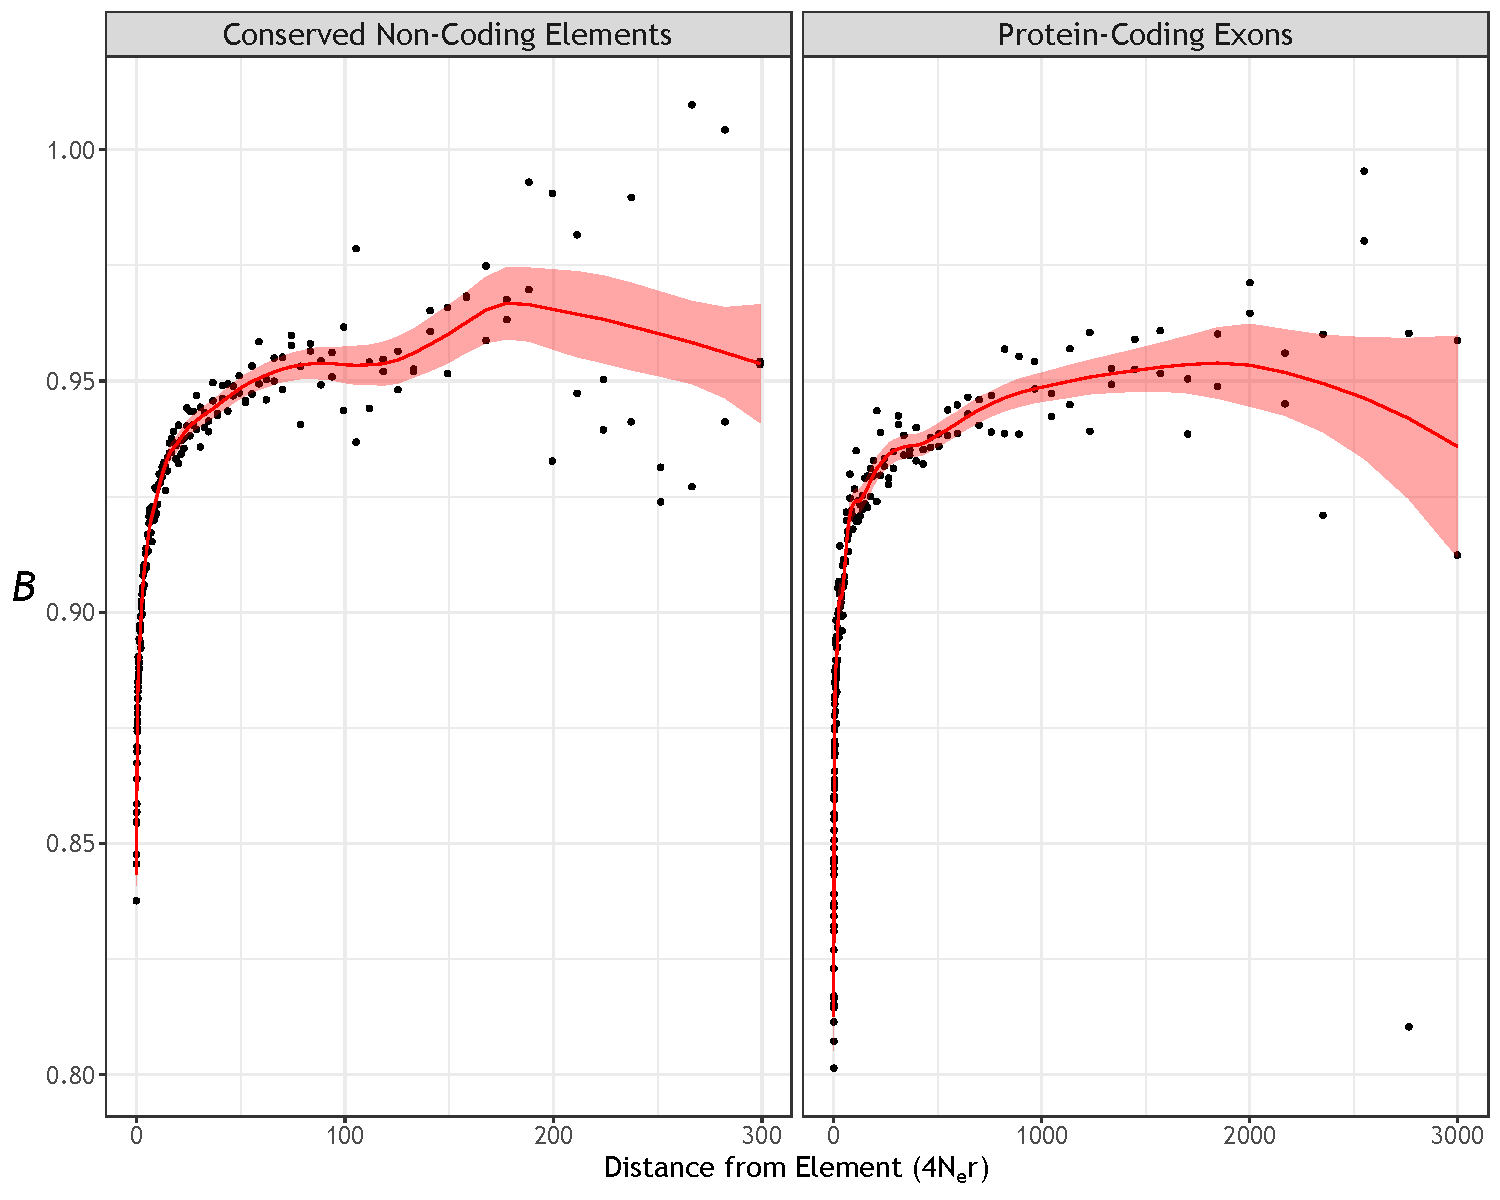
\includegraphics[width=\textwidth]{\dir/chapter4Appendix/figures/BGSplotLoess.pdf}}
 \caption{Reductions in diversity around protein-coding exons and CNEs in simulations. Red lines are Loess curves fitted to the data with a span of 0.2, the ribbons are 95\% prediction intervals}.
 
 \label{fig:BGSLoess}
\end{figure}

\begin{figure}[H]
   \centering      
   \noindent\makebox[\textwidth]{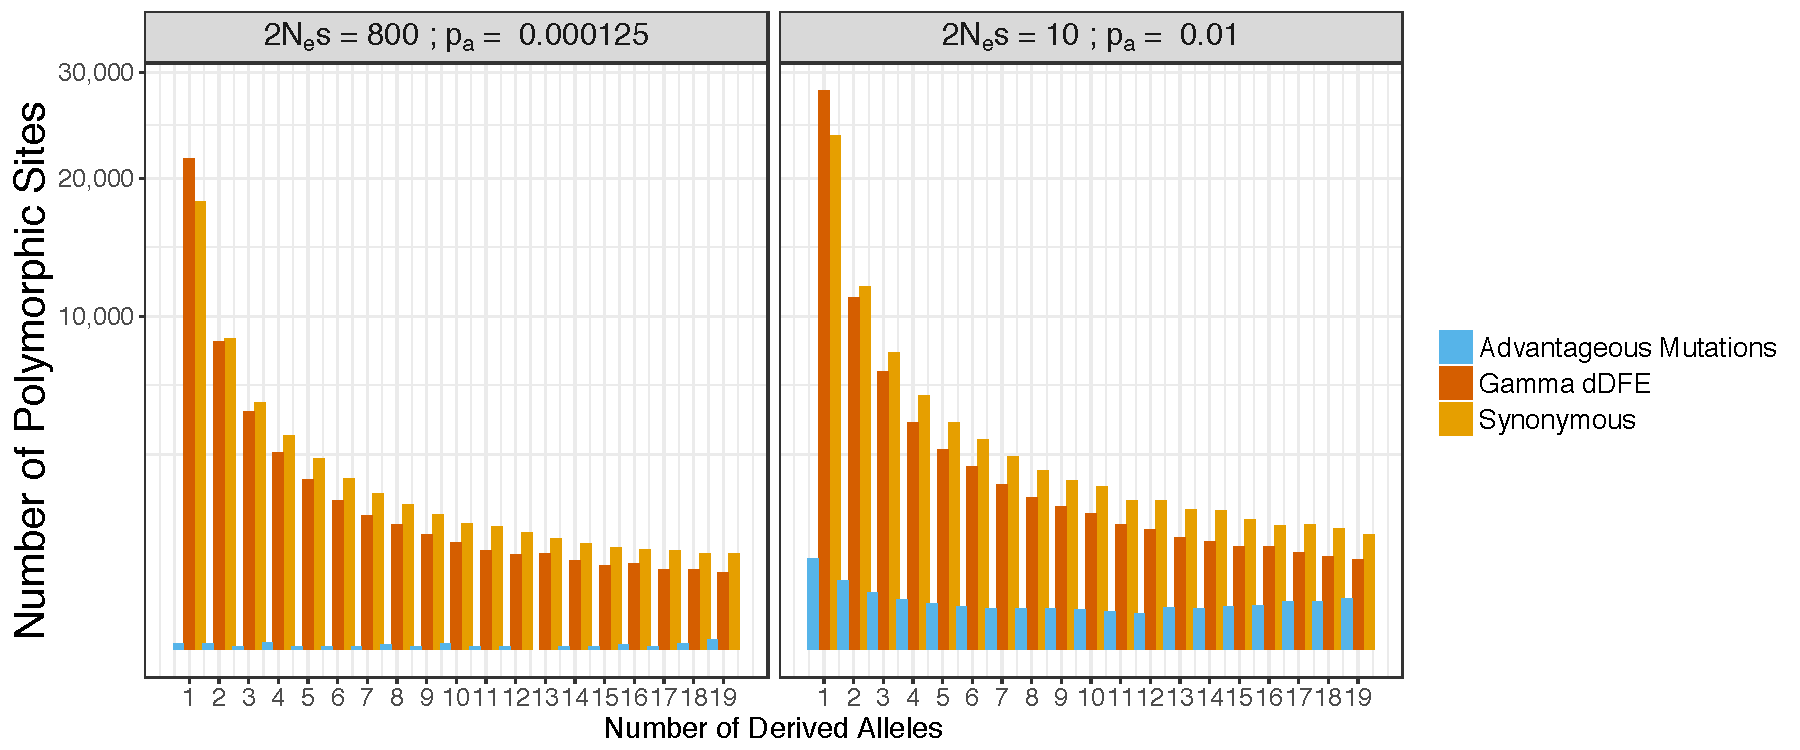
\includegraphics[width=\textwidth]{\dir/chapter4Appendix/figures/SFSplot.pdf}}
 \caption{Examples of the unfolded site frequency spectra obtained from simulated data.}.
 
 \label{fig:SFSexample}
\end{figure}


\begin{table}[H]
   \centering
      \begin{threeparttable}[b]

\caption{The effect of gene conversion on parameter estimates. Values shown were obtained assuming the \textit{castaneus} map and two classes of advantageous mutational effects. Standard errors are shown below point estimates in square brackets.}

\begin{tabular}{ccccccc}

\toprule
Element 		&      GC\tnote{a}  &          $\gamma_{a,1}$ &            $p_{a,1}$ &       $\gamma_{a,1}$ &      $p_{a,2}$ \\
\midrule
   \multirow{6}{*}{Exon} &    \multirow{2}{*}{None} &   8,340&  2.27 x $10^{-5}$ &   20.9&  0.0215\\
             &      &    [673]&  [2.30 x $10^{-6}$]&    [3.36]&  [0.00499]          \\
 	      	 &  \multirow{2}{*}{Low}  &   8,470 &  2.22 x $10^{-5}$ &   22.4&  0.0202\\
             &      &    [672]&  [2.21 x $10^{-6}$]&    [3.39]&  [0.00438]\\
   		     &    \multirow{2}{*}{High}  &  15,000 &  9.00 x $10^{-6}$ &  174&  0.00322\\
             &      &   [1,030] &  [8.24 x $10^{-7}$] &    [7.07] &  [0.000158]          \\ \hdashline
    \multirow{6}{*}{CNE}		 &    \multirow{2}{*}{None}  &    430&  1.13 x $10^{-3}$ &   14.0&  0.0300\\
             &      &     [23.1] &  [9.67 x $10^{-5}$] &    [3.50] &  [0.00956]      \\
     		 &  \multirow{2}{*}{Low}  &    432 &  1.12 x $10^{-3}$ &   14.5&  0.0298\\
             &      &     [21.2]&  [8.86 x $10^{-5}$] &    [3.17] &  [0.00822]\\
     		&    \multirow{2}{*}{High}  &    550 &  1.40 x $10^{-3}$ &   73.5&  0.00474          \\
            &      &     [26.7] &  [1.39 x $10^{-4}$] &   [15.4] &  [0.000741]          \\
\bottomrule
\end{tabular}

   \begin{tablenotes}
     \item[a] Denotes the gene conversion parameters used. $None$ - No GC, $Low$ - $\kappa$ = 0.102, $High$ - $\kappa$ = 12.0. The mean tract length was set to 144bp across all analyses.
   \end{tablenotes}
  \label{tab:GeneConversion}

    \end{threeparttable}

\end{table}


\begin{table}[H]
   \centering
\begin{adjustbox}{max width=\textwidth}
   \begin{threeparttable}[b]
\caption{The effect of background selection ($BGS$) on estimates of positive selection parameters obtained by fitting the troughs in diversity. Values obtained assuming the \textit{castaneus} map and the gene conversion parameters of \cite{RN263} are shown. The difference in AIC between the full model and a model assuming that BGS does not contribute to the observed troughs }


\begin{tabular}{ccccccc}
\toprule
       Element & BGS & $\Delta AIC$ &  $\gamma_{a,1}$ &      $p_{a,1}$ &       $\gamma_{a,2}$ &      $p_{a,2}$  \\
\midrule
\multirow{2}{*}{Exon}    & - &  65.5 & 18,900 [1,510]   &  0.0000130 [0.000001] &  62.8 [9.46] &  0.00584 [0.00115] \\
 					    & + & -    &  8,470  [672]   &  0.0000220 [0.000002] &  22.3 [3.39] &  0.02020   [0.00438] \\ \hdashline
 \multirow{2}{*}{CNE}   & - &   109 &   1,460 [134]   &  0.000126 [0.000018] &  68.2  [9.73] &  0.00377 [0.000561] \\
                        & + & -    &    432  [21.2] &  0.001120 [0.000089] &  14.5 [3.17] &  0.0298   [0.00822] \\
\bottomrule
\end{tabular}
  \label{tab:BGSeffect}

\end{threeparttable}
\end{adjustbox}

\end{table}


\begin{table}
   \centering
   \begin{threeparttable}[b]
\caption{Parameters of the distribution of fitness effects for harmful mutations obtained by analysis of the uSFS. Simulated values were $\beta = 0.20$ and $\hat{\gamma_d} = -2000$  }

\begin{tabular}{cccccc}
\toprule
$\gamma_a$ & $p_a$ & Divergence\tnote{a} & Full DFE\tnote{b} & $\beta$\tnote{c} & $\hat{\gamma_d}$ \tnote{d} \\
\midrule
 \multirow{4}{*}{10}&\multirow{4}{*}{0.01000}&        + &        + &  0.203 [0.190 - 0.231] &  -865 [-1120 -  -561] \\
 &&        + &        - &  0.135 [0.127 - 0.140] & -6860 [-10100 -  -4850] \\
 &&        - &        + &  0.217 [0.190 - 0.270] &  -755 [-110000 -  -483] \\
 &&        - &        - &  0.175 [0.166 - 0.184] & -1550 [-2100 -  -1180] \\ \hline
 \multirow{4}{*}{20}&\multirow{4}{*}{0.00500}&        + &        + &  0.199 [0.184 - 0.212] &  -974 [-1390 -  -744] \\
 &&        + &        - &  0.132 [0.125 - 0.142] & -8480 [-13200 -  -5030] \\
 &&        - &        + &  0.199 [0.187 - 0.226] & -9831 [-1330 -  -676] \\
 &&        - &        - &  0.176 [0.168 - 0.183] & -1620 [-2040 -  -1230] \\ \hline
 \multirow{4}{*}{50}&\multirow{4}{*}{0.00200}&        + &        + &  0.199 [0.179 - 0.210] &  -979 [-1680 -  -740] \\
 &&        + &        - &  0.136 [0.130 - 0.144] & -7260 [-11100 -  -4930] \\
 &&        - &        + &  0.199 [0.187 - 0.215] &  -944 [-1350 -  -739] \\
   &&      - &        - &  0.186 [0.177 - 0.195] & -1220 [-1640 -  -986] \\ \hline
      \multirow{4}{*}{100}&\multirow{4}{*}{0.00100}&   + &        + &  0.195 [0.175 - 0.210] &  -952 [-1780 -  -661] \\
       &&  + &        - &  0.137 [0.129 - 0.144] & -5980 [-9350 -  -4140] \\
         &&- &        + &  0.193 [0.184 - 0.271] &  -953 [-1270 -  -637] \\
&&         - &        - &  0.189 [0.182 - 0.199] & -1040 [-1310 -  -790] \\ \hline
   \multirow{4}{*}{200}&\multirow{4}{*}{0.00050}&       + &        + &  0.197 [0.174 - 0.210] & -1040 [-2060 -  -748] \\
    &&     + &        - &  0.136 [0.130 - 0.144] & -7470 [-10700 -  -5100] \\
      &&   - &        + &  0.207 [0.187 - 0.353] &  -927 [-1320 -  -498] \\
        && - &        - &  0.190 [0.183 - 0.199] & -1160 [-1470 -  -917] \\ \hline
 \multirow{4}{*}{400}&\multirow{4}{*}{0.00025}&         + &        + &  0.209 [0.192 - 0.224] &  -745 [-1180 -  -558] \\
  &&       + &        - &  0.148 [0.141 - 0.156] & -4010 [-5910 -  -2810] \\
    &&     - &        + &  0.210 [0.199 - 0.229] &  -727 [-939 -  -541] \\
      &&   - &        - &  0.202 [0.193 - 0.212] &  -840 [-1040 -  -660] \\ \hline
         \multirow{4}{*}{800}&\multirow{4}{*}{0.0001}&  + &        + &  0.210 [0.181 - 0.218] &  -798 [-1500 -  -592] \\
&&         + &        - &  0.148 [0.139 - 0.157] & -3890 [-6000 -  -2720] \\
  &&       - &        + &  0.205 [0.193 - 0.236] &  -804 [-1020 -  -543] \\
    &&     - &        - &  0.198 [0.189 - 0.209] &  -889 [-1130 -  -693] \\
\bottomrule
\end{tabular}

   \begin{tablenotes}
     \item[a] +/- indicates whether or not divergence was included when analysing the uSFS
     \item[b] +/- indicates whether or not advantageous mutation parameters were inferred
     \item[c] The shape parameter of the gamma distribution of deleterious fitness effects
     \item[d] Mean strength of selection of a new harmful mutation
   \end{tablenotes}
     \label{tab:dDFE}

  \end{threeparttable}
  
\end{table}



